\section{Теоретичні основи ООП: Інкапсуляція та модифікатори доступу}

\subsection{Концепція інкапсуляції та приховання реалізації}

Об'єктно-орієнтоване програмування базується на представленні програми як сукупності 
взаємодіючих об'єктів. Одним із фундаментальних принципів цієї парадигми 
є \textbf{інкапсуляція} — процес відокремлення один від одного елементів об'єкта, 
що визначають його внутрішній устрій (реалізацію) від Його зовнішньої поведінки 
(інтерфейсу). 

У межах виконання лабораторної роботи інкапсуляція розглядається як захисна оболонка, 
яка оберігає дані об'єкта від неконтрольованого прямого втручання з боку зовнішнього коду. 
Взаємодія з об'єктами здійснюється виключно через чітко визначений публічний контракт 
методів (інтерфейс), що дозволяє локалізувати частини реалізації системи, які можуть 
зазнати змін у майбутньому (наприклад, повна заміна внутрішньої структури кошика зі 
стека на чергу без зміни зовнішнього коду додатку).

\subsection{Модифікатори доступу в мові Java}

Для практичної реалізації механізму інкапсуляції в мові Java використовується система 
рівнів захисту полів та методів класів за допомогою модифікаторів доступу:
\begin{itemize}
    \item \textbf{\texttt{private}:} 
    Найсуворіший рівень доступу. Члени класу, оголошені з цим модифікатором, доступні 
    лише методам та конструкторам всередині цього ж класу. Закриття полів (\texttt{name}, 
    \texttt{price}, \texttt{stack}) забезпечує повний контроль над станом об'єкта.
    \item \textbf{За замовчуванням (\texttt{package-private}):} 
    Рівень доступу, який застосовується автоматично за відсутності модифікатора. 
    Елементи доступні будь-яким іншим класам, що знаходяться у тому самому пакеті.
    \item \textbf{\texttt{protected}:} 
    Забезпечує видимість членів класу для всіх компонентів всередині поточного пакету, 
    а також для підкласів (нащадків) в інших зовнішніх пакетах.
    \item \textbf{\texttt{public}:} 
    Повністю відкритий доступ. Члени класу доступні для будь-яких зовнішніх методів 
    та класів як у поточному, так і в інших пакетах додатка. Складають зовнішній інтерфейс 
    взаємодії об'єкта.
\end{itemize}

\subsection{Модифікатори доступу та анотація @Override в архітектурі інтерфейсів}

Особливе місце в реалізації об'єктно-орієнтованого поліморфізму посідає службовий маркер 
компілятора — анотація \textbf{\texttt{@Override}}. На відміну від мови C++, де для 
створення віртуальних функцій у базовому класі обов'язково використовується ключове слово 
\texttt{virtual}, у Java всі нестатичні методи є віртуальними за замовчуванням. 

У розроблених компонентах \texttt{StackCart} та \texttt{QueueCart} анотація \texttt{@Override} 
застосована перед кожним методом, що приходить із контракту інтерфейсу \texttt{Cart}. Функціональне 
призначення цієї директиви полягає в наступному:
\begin{enumerate}
    \item \textbf{Контроль сигнатури:} 
    Вона примусово наказує компілятору перевірити, чи дійсно метод з такою самою назвою та 
    параметрами існує в інтерфейсі.
    \item \textbf{Захист від помилок розробника:} 
    Якщо під час написання коду в дочірньому класі буде допущено друкарську помилку 
    (опечатку) у назві методу, компілятор зупинить збирання проєкту з помилкою невідповідності, 
    що запобігає виникненню прихованих багів непрацюючого поліморфізму.

\end{enumerate}


\subsection{Роль конструкторів та ключового слова \texttt{this}}

Конструктор є спеціальним методом класу, який автоматично викликається оператором \texttt{new} 
під час створення нового екземпляра для ініціалізації його початкового стану. Конструктор не 
має типу повертаємого значення, а його ім'я строго збігається з назвою класу. 

У розроблених компонентах (\texttt{Item}, \texttt{StackCart}, \texttt{QueueCart}) імена 
вхідних аргументів конструкторів збігаються з іменами внутрішніх змінних екземпляра. Для 
розв'язання конфлікту імен застосовано приховане посилання на поточний об'єкт за допомогою 
ключового слова \textbf{\texttt{this}} (наприклад, \texttt{this.price = price}), що дозволяє 
компилятору чітко розрізняти локальні параметри методу від полів об'єкта у кучі (\text{Heap}).

\subsection{Об'єктно-орієнтована архітектура та UML-діаграма класів}

Для детального аналізу взаємодії створених компонентів програми було розроблено архітектурну 
UML-діаграму класів у середовищі Draw.io. Спроектована структура наочно демонструє застосування 
ключових принципів об'єктно-орієнтованого програмування, зокрема інкапсуляції та поліморфізму 
через інтерфейсні контракти.

\begin{figure}[H]
    \centering
    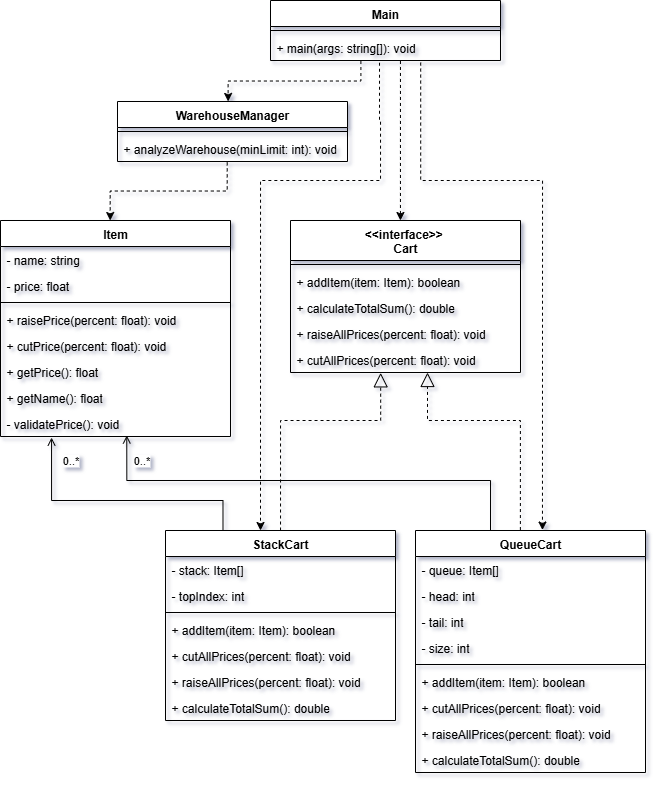
\includegraphics[width=0.85\textwidth]{screenshots/uml_diagram.png}
    \caption{UML-діаграма взаємодії класів та інтерфейсів розробленого додатка}
    \label{fig:uml_diagram}
\end{figure}

Основними архітектурними зв'язками на схемі (рис.~\ref{fig:uml_diagram}) є:
\begin{itemize}
    \item \textbf{Відношення реалізації (Realization):} 
    Класи \texttt{StackCart} та \texttt{QueueCart} пов'язані з інтерфейсом \texttt{Cart} 
    пунктирними стрілками з білим трикутним наконечником. Це показує, що обидва компоненти 
    зобов'язані повністю виконати публічний контракт методів, приховуючи власну внутрішню 
    логіку (стек або чергу).
    \item \textbf{Відношення асоціації (Association):} 
    Класи кошиків посилаються на сутність \texttt{Item}, оскільки містять всередині себе масиви 
    об'єктів товарів, реалізуючи відношення агрегації типу «один до багатьох» (\texttt{0..*}).
    \item \textbf{Відношення залежності (Dependency):} 
    Клас \texttt{WarehouseManager} (Індивідуальний варіант №7 з фійлу лаб2-2.docx ) та головний 
    файл \texttt{Main} використовують класи сутностей для ініціалізації та виконання аналітичних 
    розрахунків.
\end{itemize}